\chapter{Literature Review}
\label{sec:review}
% \newcommand{\sectionbreak}{\clearpage}
\section{Introduction}
The vast majority of mobile platforms and unmanned vehicles currently in use are non-holonomic \cite{sanchez-orta_aerial_2020}. They only have one or two independent degrees of freedom. As a result, its manoeuvrability is restricted, and it frequently necessitates a large amount of space to control functions like turning and parking \cite{bremer_problems_2010}. This is visible when a car wants to turn $180^0$. We improve a vehicle's manoeuvrability by increasing its degrees of freedom. It can take many complex paths that conventional nonholonomic vehicles find difficult or impossible to follow. The relationship between a robot's controllable and total degrees of freedom is referred to as holonomic \cite{yun_unified_1998}. Any mobile platform with three independent degrees of freedom in a plane is referred to as a holonomic platform. The robot is said to be holonomic if the controllable degree of freedom equals the total degree of freedom \cite{thompson_chapter_2017}. In contrast to car-type vehicles, which must turn or change orientation when moving, independent degrees of freedom indicates that it can change its orientation or position without affecting other motions. A holonomic drive is demonstrated by a robot built on castor wheels or Omni-wheels, which can freely move in any direction and has controllable degrees of freedom equal to total degrees of freedom.

\subsection{Mobile Platforms}
Researchers have been working on omnidirectional wheeled mobile robots for the last three decades. There are also legged mobile robots that can move in both omnidirectional and holonomic directions. Legged mobile platforms have the advantage of being highly adaptable to uneven terrain, having low soil interaction, and being able to perform tasks in congested and narrow areas. Despite this, their slow mobility, low payload-to-mechanic weight ratio, and complex design and control make them difficult to locate.

\subsection{Caster wheel}
A castor or caster wheel is a relatively free-rolling ,not powered, small undriven wheel. They are designed to be attached to the bottom of a larger object, to enable easy movement across a floor or other hard surface. Castor wheels are manufactured in either a single-wheel, double-wheel, or compound-wheel configuration.
\par
Most castors are used simply to make a heavy or cumbersome piece of furniture or machinery - the vehicle - easier to move. Affixing small, unobtrusive wheels to the bottom of any large or bulky item is a great way to make it more mobile in certain scenarios. In most cases, they are attached to the underside of the vehicle via a fixed top plate, from which the wheel assembly hangs.
\par
When choosing the type of casters to use in an application, weight considerations need to be considered depending on the load the casters will be required to move. To achieve this, we need to consider the weight of the item being supported as shown by equation \ref{eq:1}.

\begin{equation} \label{eq:1}
total\:load\:capacity = individual\:weight\:rating * number\:of\:wheels
\end{equation}

The total load-bearing capacity of your castors should always be at least 30\% higher than the total weight of the item when fully loaded, to give a sufficient safety margin. Another consideration to take into account is the type of surface the castors will be moving on. These surfaces are either flat and smooth that can accommodate small wheels or rougher surfaces that require wheels with larger diameters.
\par
There are several types of caster wheels each suited to a different application. The most common casters are shown in Figure \ref{fig:casterwheels}
\vspace{5mm}
\begin{figure}[H]
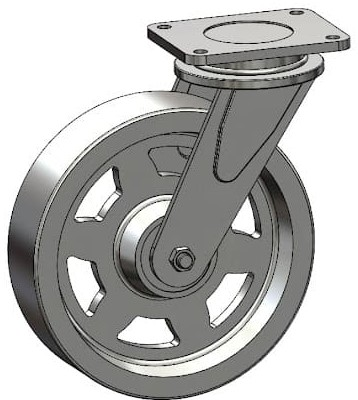
\includegraphics[scale=0.45]{Figures/ferrous-caster-wheel.jpg} 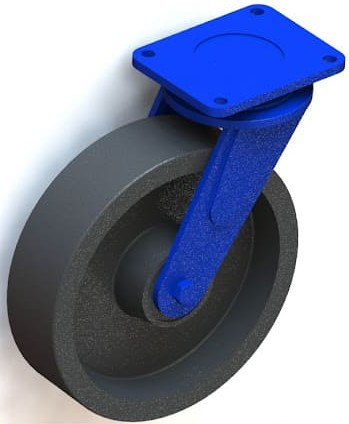
\includegraphics[scale=0.45]{Figures/synthetic-tread-wheels.jpg} 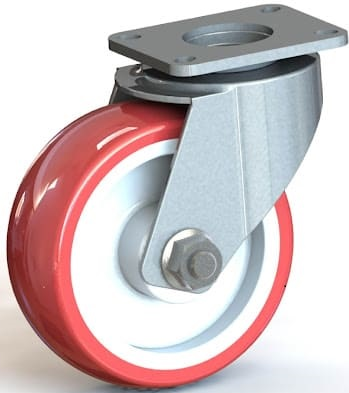
\includegraphics[scale=0.45]{Figures/polyurethane-caster-wheel.png}\centering
\caption[Caster Wheels] {Caster Wheels \cite{noauthor_caster_nodate}.}
\label{fig:casterwheels}
\end{figure}

{\sectionbreak}
\section{Existing Technologies}
\subsection{Wheeled Vehicles}
For wheeled mobile robots, we have: conventional wheels, omnidirectional wheels, and ball wheels \cite{muir_kinematic_1987}. The conventional wheels are the ones we see on cars and trolleys every day. An omnidirectional wheel is a disk-shaped wheel with numerous conventional wheels mounted on its periphery. A ball wheel \cite{ostrovskaya_dynamics_2000,west_design_1995}, is shaped like a ball but its implementation is difficult because including an axle in the design sacrifices usable workspace. It is also difficult to provide power transmission to the wheel. For large and heavy outdoor robots, four-wheel or car-like driving mechanisms have traditionally been used. Because the non-holonomic constraints on their wheel mechanisms prevent sideways movements, these vehicles are quite restricted in their motion \cite{laumond_feasible_1986, pin_autonomous_1990, noauthor_navigation_nodate}, especially when operating in tight environments. Improved motion capabilities have been investigated in a number of research centres and demonstrated on laboratory robots. These motion capability enhancements are typically derived from the use of two independent driving wheels supplemented by casters. This allows the platform to rotate around any point but does not allow for sideways motion. Another motion can be achieved using two steerable and independently driving wheels \cite{pin_autonomous_1989}, or three steerable and coordinated driving wheels \cite{pin_autonomous_1989}. These two implementations allow for both platform rotation and sideways motion through coordinated steering of the wheels.
\par
However, in these latter systems, the controls for translational and rotational motions are not fully decoupled or independent, as very strict compatibility conditions exist between the steering and driving velocities of the wheels \cite{alexander_kinematics_1989}. To achieve the full three degrees of freedom of planar rigid body motion, these platforms must be controlled as strongly constrained systems. Furthermore, steering necessitates the rotation of the wheels around a vertical axis, which, in the case of heavy payloads or vehicles with wide tires, may result in significant wheel sliding and friction. The traditional wheel is probably the simplest and most durable of the designs.
\par
However, not all conventional wheels can provide omnidirectional motion \cite{muir_kinematic_1987, alexander_kinematics_1989, ostrovskaya_nonholonomic_1998}. It is widely accepted that caster design provides full mobility \cite{d39_structural_1996}. Mecanum wheels also achieve holonomic and omnidirectional motion by having a series of rollers attached to their circumference \cite{diegel_improved_nodate}. These rollers have an axis of rotation at $45^0$ to the plane of the wheel. The angled peripheral rollers translate a portion of the force in the rotational direction of the wheel \cite{diegel_improved_nodate}. Each mecanum wheel in a drive system has independent actuation and the resulting combination of forces to move these wheels produces a total force vector that allows the platform to move freely in any direction. Different variations of mecanum wheels depend on the number of rollers attached to individual wheels, as shown in Figure \ref{fig:differentvariationsofmecanumwheels}.

\begin{figure}[htbp]
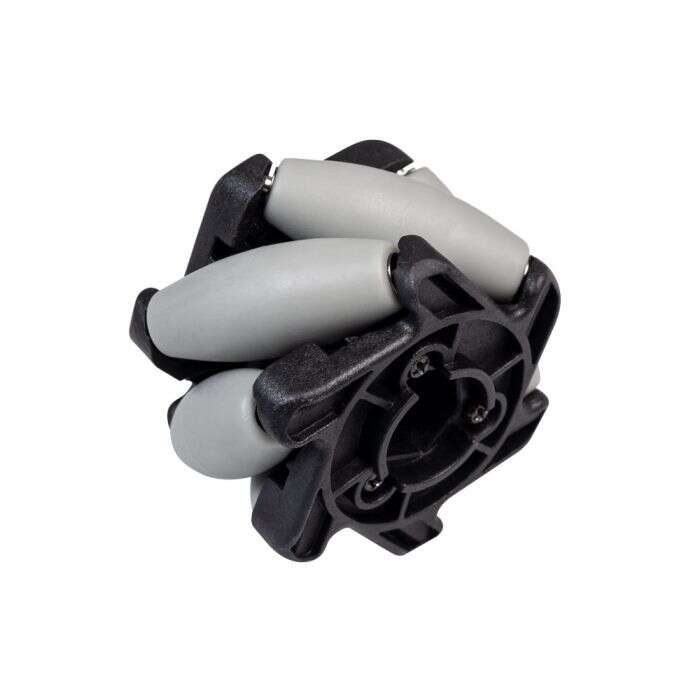
\includegraphics[scale=0.35]{Figures/mecanum1.jpg} 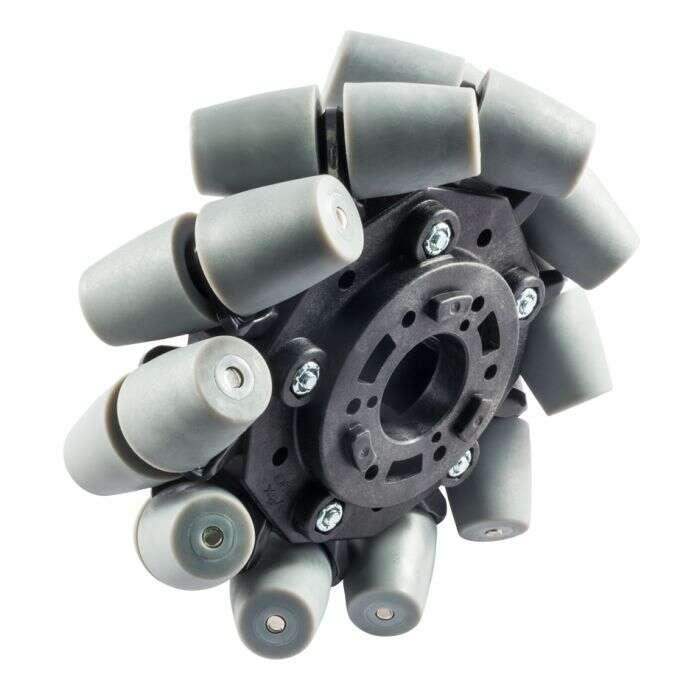
\includegraphics[scale=0.35]{Figures/mecanum2.jpg} 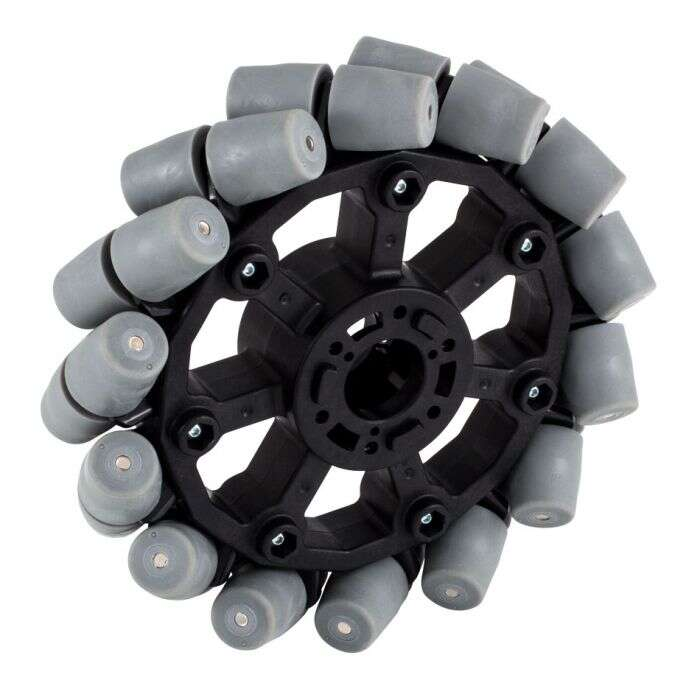
\includegraphics[scale=0.35]{Figures/mecanum3.jpg}\centering
\caption[Different variations of mecanum wheels] {Different variations of mecanum wheels \cite{diegel_improved_nodate}.}
\label{fig:differentvariationsofmecanumwheels}
\end{figure}

In the development of mecanum and other omnidirectional wheels \cite{kim_design_2001, paromtchik_practical_1994}, undesirable vibrations are frequently present in the motion due to a large number of small rollers on the wheel's periphery.

\subsection{Omnidirectional and Holonomic Motion}
A lot of design work on omnidirectional vehicles has been conducted over the years.
The earliest omnidirectional mobile vehicle to be proposed was based on introducing a methodology for the kinematic modelling of an omnidirectional wheeled mobile robot equipped with four omnidirectional wheels which were based on passive rollers arranged in an overlapping way \cite{javier_moreno_design_2016}. These wheels were positioned in pairs on the same axle but with opposite orientations. Another proposal by Wada and Mori \cite{wada_holonomic_1996} presented a new type of holonomic mobile robot which was equipped with steerable and coordinated driving wheels using conventional tires to provide an omnidirectional capability by actuating the wheels axis and a steering axis independently. In another paper by Javier Moreno, Eduard Clotet, and others design \cite{javier_moreno_design_2016} validate a three-wheel holonomic motion system for an assistant personal robot. The paper analyses the kinematics of the motion system and validates the estimation of the trajectory by comparing the displacement estimated with the internal odometry of the motors and the displacement estimated with a \ac{SLAM} procedure based on \ac{LIDAR} information . 

{\sectionbreak}
\section{Remote Control Strategies}
The remote-controlled system employs a monitor and a control device. The operator controls the remote-controlled robot with the control device while keeping an eye on the monitor, which displays visual data from the visual sensors. Expert operators who understand and are capable of training the remote-controlled robot are required to operate flexibly. Thus, operating a remote-controlled robot is difficult and may result in operational errors. This is because using a monitor that only displays visual information makes it difficult for the operator to understand real-world environmental situations. As a result, numerous stages of training are required for the operator to recognise the surroundings from visual information for expert operation \cite{masaki_remote-controlled_2022}.

Methods for improving the operability of the remote-controlled robot in terms of the mechanical design of the control device and the operation assist control method have been reported. Wireless control strategy advanced multioperability of robots \cite{almali_wireless_2015} but they are just a network to which control strategies connect to. This study proposes a remote-controlled method with an \ac{API} to improve the diversity of remote control applications. 

By combining human intuitions with the robot's motor capabilities, a motion-based control interface enables flexible robot operations in hazardous environments. It is more difficult to design a motion interface for non-humanoid robots, such as quadrupeds or hexapods, because their motions are governed by different dynamics and control techniques.
\begin{enumerate}
    \item Supervised Learning
    \par
    They employ supervised learning and post-processing techniques to convert the acquired human motion into an equivalent robot motion with appropriate semantics. They then combine motion imitation with curriculum learning to develop a control policy capable of monitoring a re-targeted reference. The authors train a group of experts to improve the performance of motion re-targeting and motion imitation. They demonstrate how the new system can perform a variety of motor activities on quadrupeds, including standing, sitting, tilting, manipulating, walking, and turning. In addition, they conduct research to determine how each component affects performance.
    \item Human Motion Control
    \par
    Human motion control allows human movements to control the robot body directly. Motion control systems relieve the human operator of the need to use traditional control devices (such as joysticks and keyboards), allowing the operator to communicate their intentions to the robot controller more effectively. As a result, human posture-based control has received a lot of attention in robotics.
\end{enumerate}

\section{Gap Analysis}
Huge leaps have been made in the development of mobile vehicles or robots with holonomic and omnidirectional motion.
Mecanum wheels have taken center stage, and the use of rollers attached to a conventional wheel has found great applications in small-scale robots and mobile platforms.
However, these wheels cannot be applied to certain applications that involve heavy payloads or rough terrains, such as moving objects in warehouses or factory floors.
Castors are predominantly used in these areas, but it involves manual control.
This process can be automated by adding motors to castors for directional control and adding the concept of remote control. Furthermore, most automated platforms have a fixed mode of control and lack the implementation of \ac{API}s embedded in their control, which necessitates this research.